\documentclass[preprint,12pt,authoryear]{elsarticle}

% ==================================================
% Packages
% ==================================================

\usepackage{amssymb}
\usepackage{amsmath}
\usepackage{graphicx}
\usepackage[hidelinks]{hyperref}
\usepackage{placeins}

% Chinese
\usepackage{xeCJK}
\setCJKmainfont{FandolSong-Regular}
\setCJKsansfont{FandolHei-Regular}
% Tables
\usepackage{booktabs}
\usepackage{multirow}
\usepackage{longtable}
\usepackage{array}
\usepackage{chngcntr}

% Algos
\usepackage{algorithm}
\usepackage{algpseudocode}

% ==================================================
% Journal
% ==================================================

\journal{ESWA}



% ==================================================
% Document
% ==================================================

\begin{document}

\begin{frontmatter}

% ==================================================
% Title
% ==================================================
\title{HKG-RAG: An Adaptive Retrieval-Augmented Generation Framework with Hierarchical Knowledge Graphs and Multi-Agent Collaboration}

% ==================================================
% Abstract
% ==================================================

\begin{abstract}
Naive retrieval-augmented generation (RAG) built upon vector retrieval still suffers from limitations when processing queries demanding complex multi-hop reasoning or global comprehension of the knowledge base. To address these limitations, existing studies have incorporated knowledge graphs into RAG and further explored hierarchical knowledge organization, for instance via multi-level summaries. However, existing methods still face two major limitations. First, their retrieval strategies are relatively rigid, and the retrieval process lacks sufficient awareness of graph structure, making it difficult to fully exploit hierarchical knowledge organization during retrieval. Second, they exhibit limited capability for reasoning over multi-granularity knowledge and lack differentiated retrieval and reasoning strategies for queries of varying granularity. To address these challenges, we propose HKG-RAG, an adaptive RAG framework that integrates hierarchical knowledge graphs with multi-agent collaboration. HKG-RAG constructs a hierarchical knowledge graph through document information extraction, entity--relation modeling, and document topic clustering. It further introduces a collaborative question-answering workflow consisting of a QuestionAnalysis agent, a RetrievalDecision agent, and an AnswerEvaluation agent. Guided by query characteristics, the workflow performs multi-granularity knowledge retrieval by dynamically selecting among document-chunk retrieval, entity retrieval, entity--relation retrieval, and topic retrieval, and iteratively refines its retrieval strategy based on evaluation feedback. Experiments on public question-answering benchmark datasets spanning four domains and a self-constructed private-domain dataset demonstrate that HKG-RAG effectively improves question-answering quality.The source code and dataset will be made publicly available upon publication.
% ==================================================
% The source code and dataset are publicly available at GitHub:
% \url{https://github.com/WJQ-7/HKG-RAG}.
% ==================================================
\end{abstract}

% ==================================================
% Keywords
% ==================================================

%% Keywords
\begin{keyword}
Retrieval-Augmented Generation
\sep Hierarchical Knowledge Graph
\sep Multi-Agent Collaboration
\sep Private-Domain Question Answering
\end{keyword}

\end{frontmatter}


% ==================================================
% 1. Introduction
% ==================================================

\section{Introduction}
\label{sec:introduction}
In recent years, large language models (LLMs) \citep{radford2019language,brown2020language}
have achieved remarkable progress in natural language understanding and text generation.
However, when relying solely on their internal knowledge, LLMs are prone to factual errors
and hallucinations \citep{li2024dawn}.
Retrieval-augmented generation (RAG) \citep{lewis2020retrieval} provides an effective
approach to mitigating these issues. Its core idea is to retrieve relevant information
from external knowledge sources and provide it as contextual evidence to the generative model, thereby improving its performance on knowledge-intensive tasks \citep{guu2020realm,izacard2021leveraging}.
Furthermore, RAG has been widely applied to domain-specific knowledge tasks, where domain databases or knowledge sources are incorporated to provide large language models with external domain knowledge \citep{tu2024reval}. Meanwhile, external knowledge retrieval can also supplement the model with up-to-date knowledge\citep{zhao2026retrieval}, giving RAG clear advantages in domains where knowledge evolves rapidly.
However, naive RAG retrieves relevant document chunks from massive corpora through semantic vector similarity matching. Nevertheless, it merely considers semantic similarity between queries and knowledge-base fragments rather than ensuring genuine content relevance. In addition, the flat knowledge organization scheme cannot capture high-level semantic abstractions of raw documents, leading to semantic-level mismatches and deteriorated response quality when handling abstract queries \citep{sarthi2024raptor}.

To overcome the inherent limitations of semantic-vector-based unstructured retrieval, researchers have explored incorporating knowledge graphs into RAG frameworks. To address corpus-level global and abstract queries that naive RAG struggles to handle effectively, GraphRAG \citep{edge2024graphrag} constructs a knowledge graph by extracting entities and relations from source documents, organizes the graph into hierarchical communities through community detection, and generates summaries for these communities to support global information aggregation and question answering. Although this approach improves the ability to answer global and abstract queries, its global search relies on aggregating information from multiple community summaries, some of which may provide limited relevance to the current query, thereby increasing retrieval and generation overhead.
Subsequently, LightRAG \citep{guo2025lightrag} incorporates graph structures into text indexing and retrieval and introduces a dual-level retrieval mechanism for low-level and high-level knowledge discovery, improving retrieval efficiency and accuracy. However, its dual-level mechanism is mainly reflected in the retrieval strategy, whereas the underlying knowledge graph remains centered on entities and relations, without further organizing knowledge into an explicit hierarchical representation.
LeanRAG \citep{zhang2026leanrag} further constructs multi-level semantic summaries through entity aggregation and establishes explicit relations among aggregation-level summaries to alleviate the ``semantic island'' problem caused by disconnected high-level summary nodes. It also employs bottom-up, structure-guided retrieval to aggregate relevant knowledge across different levels.
Overall, existing methods have enhanced structured knowledge organization and retrieval through graph structures, community summaries, and hierarchical aggregation. However, their improvements mainly focus on knowledge organization or predefined retrieval mechanisms, with limited explicit awareness of query granularity and limited dynamic alignment between knowledge levels and retrieval strategies. Consequently, when handling queries of different granularities, these methods remain limited in adaptively selecting appropriate knowledge levels and retrieval strategies according to query characteristics.

To address the above challenges, we propose HKG-RAG
(Hierarchical Knowledge Graph with Retrieval-Augmented Generation), an adaptive RAG framework that integrates hierarchical knowledge graphs with multi-agent collaboration. Designed for private-domain document question answering, HKG-RAG explicitly introduces a document layer above the entity layer and further constructs a topic layer through document topic clustering, forming a three-layer knowledge graph composed of entity, document, and topic layers. While preserving the entity--relation topology to support multi-hop reasoning, the framework models document and topic entities to provide higher-level knowledge support for global and abstract queries. On this basis, a multi-agent collaboration mechanism is introduced to adaptively select appropriate knowledge levels and retrieval methods according to the query type, thereby improving the system's ability to answer queries at different granularities.

The main contributions of this work are summarized as follows:

\begin{itemize}
\item A hierarchical knowledge graph structure is proposed for private-domain document question answering. It organizes knowledge into three layers---entity, document, and topic nodes---providing a hierarchical basis for knowledge organization and retrieval across queries of different granularities.
\item A query-aware multi-agent adaptive retrieval framework is developed. It identifies query types and granularities, dynamically selects appropriate retrieval methods, and iteratively refines retrieval strategies through answer evaluation and reflection-based feedback, thereby improving retrieval and question-answering performance for multi-granularity queries.
\item We build BISTU-OfficeQA, a Chinese private-domain question-answering dataset grounded in real-world university office documents, covering university-issued notices, public announcements, and administrative regulations, and providing a realistic benchmark for evaluating retrieval and reasoning capabilities across different query granularities in private-domain scenarios.
\item An end-to-end private-domain document question-answering system integrating hierarchical knowledge graphs with multi-agent collaboration is implemented. Extensive experiments across multiple datasets and evaluation metrics demonstrate the effectiveness of HKG-RAG and its strong question-answering performance.

\end{itemize}

% ==================================================
% 2. Related Work
% ==================================================

\section{Related Work}
\label{sec:related-work}


\subsection{Retrieval-Augmented Generation}
\label{subsec:rag}
RAG systems enhance the question-answering capabilities of large language models by incorporating external knowledge sources, thereby alleviating the limitations of relying solely on the models' internal knowledge and mitigating hallucinations \citep{chan2024rqrag,fan2024survey}. Naive RAG typically retrieves a fixed number of highly relevant text chunks from an external corpus, inserts them into a prompt template as contextual information, and then feeds the augmented prompt into a large language model to generate the answer \citep{yu2024rankrag}.
However, naive RAG mainly relies on flat text-chunk similarity retrieval and therefore still faces several limitations in practical scenarios. First, textual information in real-world settings does not exist in isolation but is often interconnected. Relying solely on similarity between text chunks makes it difficult for naive RAG to represent structured relational knowledge. Second, naive RAG typically retrieves only a portion of the corpus and therefore struggles to capture comprehensive global information \citep{edge2024graphrag}.

To address the retrieval limitations of naive RAG, existing studies have explored improvements from two main perspectives: retrieval methods and knowledge organization. In terms of retrieval, traditional sparse retrieval methods such as BM25 rely on term matching \citep{robertson2009bm25}, while subsequent studies have developed dense semantic retrieval methods such as DPR \citep{karpukhin2020dpr} to improve semantic matching between queries and text passages. In terms of knowledge organization, researchers have begun to explore more structured and hierarchical representations of source documents. For example, TreeRAG \citep{tao2025treerag} constructs a hierarchical knowledge structure through tree-based chunking and employs bidirectional traversal retrieval to access information at different levels. However, such hierarchical text-organization methods still primarily organize knowledge around textual content and its hierarchical structure, without explicitly modeling entities and their relations. As a result, they may remain limited when handling queries that require reasoning over complex relational dependencies and multi-hop connections. This limitation has motivated increasing research interest in knowledge-graph-based RAG.
\subsection{Knowledge Graph Based RAG}
\label{subsec:graph-rag}
Knowledge-graph-based RAG explicitly models entities and their relations to organize external knowledge into structured graphs, while exploiting relational information during retrieval to provide large language models with more comprehensive contextual support, thereby enhancing their capabilities for complex question answering and multi-hop reasoning \citep{peng2025graphrag}. GraphRAG \citep{edge2024graphrag} targets the limitations of naive RAG in handling global and abstract queries. It employs large language models to extract entities and relations from source documents to construct a knowledge graph, applies the Leiden algorithm to organize the graph into hierarchical communities, and generates summaries for individual communities. During global retrieval, GraphRAG generates partial responses based on multiple community summaries and subsequently aggregates them to support corpus-level understanding and question answering. LightRAG \citep{guo2025lightrag} introduces a dual-level retrieval framework to balance local and global information, retrieving knowledge at both levels to support question answering. However, its dual-level mechanism is mainly reflected in the retrieval strategy, while the underlying knowledge graph remains primarily composed of entities and relations. HiRAG \citep{huang2025hirag} further constructs a hierarchical knowledge graph by semantically clustering lower-level entities and generating higher-level summary entities, allowing different levels to represent knowledge at different granularities while enhancing the connectivity among semantically related entities through cross-level associations. LeanRAG \citep{zhang2026leanrag} further establishes explicit relations among aggregation-level summary nodes to alleviate the “semantic island” problem caused by isolated high-level summaries, and adopts a bottom-up retrieval strategy to enable knowledge expansion across hierarchical levels while reducing retrieval redundancy.

Overall, existing knowledge-graph-based RAG methods mainly improve knowledge organization through community detection, hierarchical clustering, and graph expansion, gradually evolving from entity--relation representations toward multi-level structures. However, they differ in hierarchy construction, node types, and retrieval mechanisms. As summarized in Table 1, most existing methods focus on graph organization while relying on relatively fixed retrieval strategies, with limited ability to adaptively select appropriate knowledge levels and retrieval methods for different query types.
\begin{table}[t]
\centering
\renewcommand{\arraystretch}{1.15}

\resizebox{\linewidth}{!}{
\begin{tabular}{lccccc}
\toprule

\multirow{2}{*}{Method}
& \multirow{2}{*}{KG}
& Hierarchical Knowledge
& \multirow{2}{*}{Multi-Agent}
& Adaptive
& \multirow{2}{*}{Node Types} \\

& & Organization
& & Retrieval
& \\

\midrule

GraphRAG
& $\checkmark$
& $\checkmark$
& $\times$
& $\times$
& Entity \\

LightRAG
& $\checkmark$
& $\times$
& $\times$
& $\times$
& Entity \\

HiRAG
& $\checkmark$
& $\checkmark$
& $\times$
& $\times$
& Entity, Summary Entity \\

LeanRAG
& $\checkmark$
& $\checkmark$
& $\times$
& $\times$
& Entity, Summary Entity \\

\textbf{HKG-RAG}
& $\checkmark$
& $\checkmark$
& $\checkmark$
& $\checkmark$
& Entity, Document, Topic \\

\bottomrule
\end{tabular}
}

\caption{Comparison of HKG-RAG with representative graph-based RAG methods.}
\label{tab:graph_rag_comparison}
\end{table}

\subsection{Multi-Agent Based RAG}
\label{subsec:multi-agent-rag}
As large language models (LLMs) continue to improve their capabilities in planning, reasoning, and tool use, researchers have introduced agent mechanisms into RAG, giving rise to Agentic Retrieval-Augmented Generation (Agentic RAG) \citep{ravuru2024agentic}. Compared with traditional RAG systems that rely on relatively fixed retrieval pipelines, Agentic RAG can autonomously make retrieval decisions, invoke tools, and adjust its strategy according to the query and current task state, thereby improving multi-step retrieval and complex problem solving.

According to the number of agents involved in collaboration, Agentic RAG can be categorized into single-agent and multi-agent architectures. In single-agent architectures, a single agent typically performs retrieval decision-making and information integration. For example, Search-o1 \citep{li2025searcho1} autonomously identifies knowledge gaps during reasoning and dynamically retrieves external knowledge to support subsequent reasoning. For more complex tasks, multi-agent systems \citep{guo2024multiagents,wu2024autogen} employ role specialization, information exchange, and collaborative decision-making to jointly accomplish complex tasks.

More recently, multi-agent mechanisms have been increasingly incorporated into RAG. MAIN-RAG \cite{chang2025mainrag} employs multiple agents to collaboratively filter retrieved documents, while DRAG \citep{hu2025drag} uses multi-agent debate to improve the reliability of generated responses. Graph Counselor \citep{gao2025graphcounselor} further employs multiple agents to dynamically select graph operations and integrates reflection mechanisms to enhance graph-based reasoning. While these methods mainly focus on retrieval filtering, answer reliability, or graph reasoning, the proposed HKG-RAG further considers the alignment between query granularity and knowledge granularity. It integrates multi-agent collaboration with a hierarchical knowledge graph and dynamically adjusts retrieval strategies through feedback from answer evaluation.


% ==================================================
% 3. HKG-RAG
% ==================================================

\section{HKG-RAG}
\label{sec:hkg-rag}
To address the limitations of existing methods in retrieval adaptivity, structural awareness, and the alignment between knowledge granularity and query granularity, we propose HKG-RAG, whose overall framework is illustrated in Fig. 1. HKG-RAG consists of two stages: pre-construction and question answering. In the pre-construction stage, document information extraction, hierarchical knowledge graph construction, and vector index establishment are performed. In the question-answering stage, the QuestionAnalysis, RetrievalDecision, and AnswerEvaluation agents collaborate to dynamically select among four retrieval tools—document-chunk retrieval, entity retrieval, entity--relation retrieval, and topic retrieval—according to query characteristics, while iteratively refining the retrieval strategy based on evaluation feedback. By combining static hierarchical knowledge organization with dynamic adaptive retrieval, HKG-RAG enables effective alignment between query granularity and knowledge granularity, thereby improving retrieval and answer quality for complex private-domain question answering.
% Overall framework of HKG-RAG.
% Put the general description and Figure 1 here.
\begin{figure}[t]
\centering
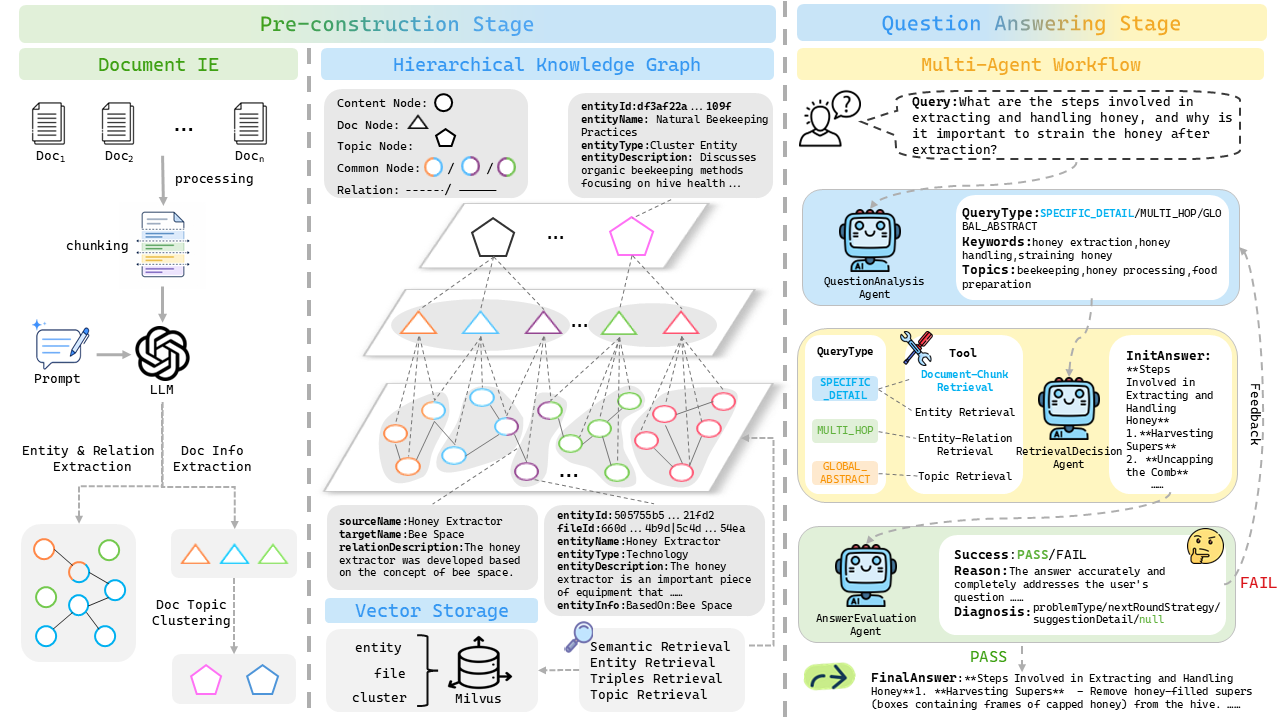
\includegraphics[width=\linewidth]{figures/hkg_rag_framework.png}
\caption{Overall framework of HKG-RAG.}
\label{fig:hkg_rag_framework}
\end{figure}

\FloatBarrier
\subsection{Hierarchical Knowledge Graph Construction}
\label{subsec:hkg-construction}

HKG-RAG organizes the source documents into a hierarchical knowledge graph consisting of an entity layer, a document layer, and a topic layer, thereby supporting knowledge retrieval and reasoning at different levels of abstraction. Specifically, the graph comprises the content entity set $E_C$, document entity set $E_D$, and topic entity set $E_T$, together with the content entity relation set $R_C$, document--content relation set $R_{DC}$, and topic--document relation set $R_{TD}$. These entity and relation sets jointly constitute the hierarchical knowledge graph $\mathcal{G}_H$, whose overall construction process is summarized in Algorithm~\ref{algo:hkg-construction}.
\begin{algorithm}[H]
\caption{Hierarchical Knowledge Graph Construction}
\label{algo:hkg-construction}
\small
\begin{algorithmic}[1]

\Require Document collection $\mathcal{D}=\{d_i\}_{i=1}^{N}$
\Ensure Hierarchical knowledge graph $\mathcal{G}_{H}$

\State
$C_i
=
\operatorname{Chunk}(d_i)
=
\{c_{ij}\}_{j=1}^{M_i},
\quad 1\leq i\leq N$

\State
$E_D
=
\{e_D^i\}_{i=1}^{N}
=
\left\{
\operatorname{Merge}_{D}
\left(
\left\{
\operatorname{Extract}_{D}(c_{ij},name_{d_i})
\right\}_{j=1}^{M_i}
\right)
\right\}_{i=1}^{N}$

\State
$T_D
=
\{t_{d_i}\}_{i=1}^{N}
=
\left\{
\operatorname{Merge}_{T}
\left(
\left\{
\operatorname{Extract}_{T}(c_{ij},name_{d_i})
\right\}_{j=1}^{M_i}
\right)
\right\}_{i=1}^{N}$
\State
$(\hat{E}_C,\hat{R}_C)
=
\bigcup_{i=1}^{N}
\bigcup_{j=1}^{M_i}
\operatorname{Extract}_{C}(c_{ij})$

\State
$E_C
=
\operatorname{DeDup}(\hat{E}_C)$

\State
$R_C
=
\operatorname{Merge}_{R}
(\hat{R}_C,E_C)$

\State
$R_{DC}
=
\bigcup_{i=1}^{N}
\left\{
(e_D^i,r,e_C^k)
\mid
e_C^k\in E_C,\;
e_C^k\text{ occurs in }d_i
\right\}$

\State
$P_T
=
\{p_T^w\}_{w=1}^{W}
=
\operatorname{DBSCAN}
\left(
\left\{
\operatorname{Embed}(t_{d_i})
\right\}_{i=1}^{N}
\right),
\quad
\bigcup_{w=1}^{W}p_T^w
=
T_D$

\State
$E_T
=
\{e_T^w\}_{w=1}^{W}
=
\left\{
\operatorname{TopicSummary}(p_T^w)
\right\}_{w=1}^{W}$

\State
$R_{TD}
=
\bigcup_{w=1}^{W}
\left\{
(e_T^w,r,e_D^i)
\mid
t_{d_i}\in p_T^w
\right\}$

\State
$\mathcal{G}_{H}
=
\left(
E_C\cup E_D\cup E_T,\,
R_C\cup R_{DC}\cup R_{TD}
\right)$

\State \Return $\mathcal{G}_{H}$

\end{algorithmic}
\end{algorithm}


\subsubsection{Document Layer Construction}

The document layer is designed to model document-level semantic information and metadata, including the title, topic, summary, publishing organization, etc. Each source document $d_i$ corresponds to a unique document node $e_D^i$, which preserves the overall context of the document and provides a document-level representation for subsequent hierarchical knowledge organization and retrieval. Its construction process is shown in Lines~1--3 of Algorithm~\ref{algo:hkg-construction}.

Given a document collection $\mathcal{D}=\{d_i\}_{i=1}^{N}$, each document $d_i$ is first divided into a set of text chunks $C_i=\{c_{ij}\}_{j=1}^{M_i}$, where $c_{ij}$ denotes the $j$-th chunk and $M_i$ denotes the number of chunks in $d_i$. For each chunk, document-level information is extracted with the document name as auxiliary context, and the results from the same document are merged to construct the document node $e_i^D$. Meanwhile, topic information is extracted from the chunks and further merged into the document-level topic $t_{d_i}$, which captures the overall semantic focus of the document. After all documents are processed, the resulting document nodes form the document node set $E_D=\{e_D^i\}_{i=1}^{N}$, while the document-level topics form the topic set $T_D=\{t_{d_i}\}_{i=1}^{N}$.

\subsubsection{Entity Layer Construction}

The entity layer models fine-grained factual knowledge and relational dependencies among content entities in the source documents, providing structured support for entity retrieval and multi-hop reasoning. Its construction process is shown in Lines~4--7 of Algorithm~\ref{algo:hkg-construction}.

Content entities and their relations are first extracted from each document chunk $c_{ij}$, yielding the raw content entity set $\hat{E}_C$ and raw relation set $\hat{R}_C$. Since the same entity may be repeatedly extracted from different chunks or documents, the extracted entities are globally disambiguated and deduplicated by identifying duplicate entities and integrating their types, attributes, and descriptions, resulting in the content entity set $E_C$. The corresponding relations are then merged according to the deduplicated entities to obtain the relation set $R_C$ (Lines~4--6). Subsequently, explicit associations are established between each document node $e_D^i$ and the content entities occurring in the corresponding document $d_i$, forming the document--content relation set $R_{DC}$ (Line~7). These cross-layer associations connect content entities with their source documents and provide structural support for subsequent retrieval and reasoning.

\subsubsection{Topic Layer Construction}
\label{subsubsec:topic-layer}

The topic layer organizes semantically similar document-level topics into higher-level topic cluster nodes to support topic retrieval and question answering. Its construction process is shown in Lines~8--10 of Algorithm~\ref{algo:hkg-construction}.

Each document-level topic $t_{d_i}$ is encoded into a semantic vector and clustered using DBSCAN \citep{ester1996density} with cosine distance, yielding the topic cluster set $P_T=\{p_T^w\}_{w=1}^{W}$ (Line~8). Each cluster $p_T^w$ is then summarized to generate a topic name $e_{T,\mathrm{name}}^w$ and a topic description $e_{T,\mathrm{desc}}^w$, which are used to construct the corresponding topic node $e_T^w$. The resulting topic nodes form the topic node set $E_T=\{e_T^w\}_{w=1}^{W}$ (Line~9). Finally, topic nodes are linked to the corresponding document nodes to form the topic--document relation set $R_{TD}$ (Line~10).

\subsection{Multi-Granularity Knowledge Retrieval}
\label{subsec:multi-granularity-retrieval}
The hierarchical knowledge graph and document corpus represent document knowledge from structured semantic relations and original textual content, respectively. Based on this organization, four tools are designed for retrieval at the document-chunk, entity, entity--relation, and topic levels, providing multi-granularity evidence for subsequent multi-agent question answering.

\subsubsection{Document Chunk Retrieval}
Document chunk retrieval uses the text chunks of the original documents as retrieval units and retrieves relevant evidence through semantic similarity matching. Given a user query $q$ and the document-chunk set $C$, both the query and each chunk are encoded into vector representations, and their semantic similarity is computed using cosine similarity:

\begin{equation}
\operatorname{Sim}_{vec}(q,c_i)
=
\frac{
\operatorname{Embed}(q)\cdot\operatorname{Embed}(c_i)
}{
\left\|\operatorname{Embed}(q)\right\|
\left\|\operatorname{Embed}(c_i)\right\|
},
\label{eq:chunk_similarity}
\end{equation}
where $q$ denotes the user query, $c_i$ denotes the $i$-th document chunk, and $\operatorname{Sim}_{vec}(q,c_i)$ denotes their semantic similarity. The chunks are ranked by similarity score, and the top-$k$ chunks are returned as the retrieval results.

\subsubsection{Entity Retrieval}
\label{subsubsec:entity-retrieval}

Entity retrieval takes the content entities in the hierarchical knowledge graph as retrieval targets and identifies relevant entities through lexical and semantic matching. Given a query $q$ containing $p$ query keywords, the query-keyword set is defined as $K_q=\{k_q^1,k_q^2,\ldots,k_q^p\}$. Hybrid retrieval is then performed over the content entity set $E_C$ for each query keyword:

\begin{equation}
E_q^C
=
\bigcup_{i=1}^{p}
\operatorname{Top}_{\ell}
\left[
\lambda s_{bm25}(k_q^i,e_{name}^j)
+
(1-\lambda)s_{vec}(k_q^i,e_{name}^j)
\right],
\quad e_j \in E_C,
\label{eq:entity_retrieval}
\end{equation}

where $e_{name}^j$ denotes the name of the $j$-th candidate content entity, $\lambda$ denotes the fusion weight, and $s_{bm25}$ and $s_{vec}$ denote the BM25 matching score and vector similarity score, respectively. $\operatorname{Top}_{\ell}$ selects the top-$\ell$ candidate entities for each query keyword according to the fused score, and $E_q^C$ denotes the union of the retrieval results for all query keywords. The attributes and descriptions of the retrieved entities are returned as entity-level evidence.

\subsubsection{Entity--Relation Retrieval}
\label{subsubsec:entity-relation-retrieval}

Entity--relation retrieval takes the candidate content entities returned by entity retrieval as the initial entities and expands along their relations in the hierarchical knowledge graph to obtain relational evidence. Given the candidate entity set $E_q$ returned by entity retrieval, the associated relational triples are retrieved from the content entity relation set $R_C$ as


\begin{equation}
\mathcal{F}_q
=
\bigcup_{e_i \in E_q}
\left\{
(e_i,r,e_j)
\mid
(e_i,r,e_j)\in R_C
\right\},
\label{eq:relation_expansion}
\end{equation}

where $R_C$ denotes the content entity relation set, $r$ denotes the relation between two content entities, and $\mathcal{F}_q$ denotes the retrieved triple set. Each retrieval performs a one-hop expansion from the current candidate entities to their neighboring entities. The retrieved neighboring entities can be further used as candidate entities for repeated retrieval, enabling progressive expansion along relational paths and providing relational evidence for multi-hop reasoning.
\subsubsection{Topic Retrieval}
\label{subsubsec:topic-retrieval}

Topic retrieval leverages the associations between the topic layer and the document layer to identify relevant topic cluster nodes through topic-level semantic matching and further obtain the corresponding documents. Given a query $q$ containing $Q$ query topics, the query-topic set is defined as
$T_q=\{t_q^i\}_{i=1}^{Q}$, where $t_q^i$ denotes the $i$-th query topic.
Each query topic is independently matched with the name and description of each
topic node in $E_T$ using vector similarity. Accordingly, the top-$\ell$ topic
nodes are retrieved from the name-based and description-based rankings as

\begin{equation}
\begin{aligned}
E_{T,i}^{\mathrm{name}}
&=
\operatorname{Top}_{\ell}
\left[
\operatorname{Sim}_{vec}
(t_q^i,e_{T,\mathrm{name}}^j)
\right], \\
E_{T,i}^{\mathrm{desc}}
&=
\operatorname{Top}_{\ell}
\left[
\operatorname{Sim}_{vec}
(t_q^i,e_{T,\mathrm{desc}}^j)
\right],
\end{aligned}
\quad e_T^j \in E_T,
\label{eq:topic_candidates}
\end{equation}

where $e_{T,\mathrm{name}}^j$ and $e_{T,\mathrm{desc}}^j$ denote the name and description of the $j$-th topic cluster node, respectively. $\operatorname{Top}_{\ell}$ selects the top-$\ell$ topic cluster nodes from $E_T$ in descending order according to the corresponding vector similarity. Accordingly, $E_{T,i}^{\mathrm{name}}$ and $E_{T,i}^{\mathrm{desc}}$ denote the candidate topic-node sets retrieved from the name and description representations for query topic $t_q^i$, respectively.

The two candidate rankings are then fused using Reciprocal Rank Fusion (RRF). Let $\operatorname{rank}_{\mathrm{name}}^{i}(e_T^j)$ and $\operatorname{rank}_{\mathrm{desc}}^{i}(e_T^j)$ denote the ranking positions of topic cluster node $e_T^j$ in the name-based and description-based retrieval results for query topic $t_q^i$, respectively. The final topic retrieval result is defined as

\begin{equation}
E_q^T
=
\bigcup_{i=1}^{Q}
\operatorname{Top}_{\ell}
\left[
\frac{1}
{\eta+\operatorname{rank}_{\mathrm{name}}^{i}(e_T^j)}
+
\frac{1}
{\eta+\operatorname{rank}_{\mathrm{desc}}^{i}(e_T^j)}
\right],
\quad
e_T^j \in
E_{T,i}^{\mathrm{name}}
\cup
E_{T,i}^{\mathrm{desc}},
\label{eq:topic_retrieval}
\end{equation}

where $\eta>0$ denotes the RRF smoothing parameter. For a topic cluster node that does not appear in one of the two retrieval results, the contribution from the corresponding ranking is treated as zero. $\operatorname{Top}_{\ell}$ selects the top-$\ell$ topic cluster nodes according to the fused RRF score, and $E_q^T$ denotes the union of the retrieval results for all query topics. The associated document nodes are then obtained through the topic--document relation set $R_{TD}$, and the corresponding document chunks are further retrieved as textual evidence.


\subsection{Adaptive Multi-Agent Collaboration for Question Answering}
\label{subsec:multi-agent-qa}

Based on the multi-granularity retrieval methods described in Section~3.2, HKG-RAG constructs a collaborative question-answering framework consisting of the QuestionAnalysis agent, RetrievalDecision agent, and AnswerEvaluation agent, as illustrated in Fig.~\ref{fig:hkg_rag_framework}. The three agents collaborate through a limited-round closed loop of ``question analysis $\rightarrow$ knowledge retrieval $\rightarrow$ answer generation $\rightarrow$ feedback evaluation.'' A cross-round reflection memory $\mathcal{M}$ is maintained to record the analysis, retrieval and answer generation, and evaluation results from previous rounds, which are subsequently used by the QuestionAnalysis agent to refine the analysis and guide the next retrieval round. The overall collaborative process is summarized in Algorithm~\ref{algo:multi-agent-qa}.

\begin{algorithm}[H]
\caption{Adaptive Multi-Agent Question Answering}
\label{algo:multi-agent-qa}
\small
\begin{algorithmic}[1]

\Require User query $q$, retrieval tool set $\mathcal{T}$, maximum round $G_{\max}$
\Ensure Final answer $a^{*}$

\State
$\mathcal{M}^{0}=\emptyset$

\For{$g=1$ to $G_{\max}$}

\State
$\mathcal{O}_{QA}^{g}
=
(q_{\mathrm{type}}^{g},K_q^{g},T_q^{g})
=
\operatorname{Agent}_{\mathrm{QuestionAnalysis}}
(q,\mathcal{M}^{g-1})$

\State
$\mathcal{O}_{RD}^{g}
=
(\mathcal{T}^{g},\mathcal{E}^{g},a^{g})
=
\operatorname{Agent}_{\mathrm{RetrievalDecision}}
(q,\mathcal{O}_{QA}^{g},\mathcal{T})$

\State
$\mathcal{O}_{AE}^{g}
=
(y^{g},f^{g})
=
\operatorname{Agent}_{\mathrm{AnswerEvaluation}}
(q,\mathcal{O}_{QA}^{g},a^{g},\mathcal{E}^{g})$

\If{$y^{g}=\mathrm{PASS}$}
    \State \Return $a^{g}$
\EndIf

\State
$\mathcal{M}^{g}
=
\operatorname{UpdateMemory}
\left(
\mathcal{M}^{g-1},
\mathcal{O}_{QA}^{g},
\mathcal{O}_{RD}^{g},
\mathcal{O}_{AE}^{g}
\right)$

\EndFor

\State \Return $a^{G_{\max}}$

\end{algorithmic}
\end{algorithm}
The QuestionAnalysis agent is responsible for interpreting the user query $q$ and generating the analysis result $\mathcal{O}_{QA}^{g}=(q_{\mathrm{type}}^{g},K_q^{g},T_q^{g})$ at round $g$ (Line~3), where $q_{\mathrm{type}}^{g}$, $K_q^{g}$, and $T_q^{g}$ denote the query type, retrieval keywords, and query topics, respectively. The query type is categorized as \texttt{SPECIFIC\_DETAIL}, \texttt{MULTI\_HOP}, or \texttt{GLOBAL\_ABSTRACT}. In non-initial rounds, the agent incorporates the cross-round reflection memory $\mathcal{M}^{g-1}$ to re-examine the query type and retrieval cues, and adjusts the query classification, keyword extraction, or topic selection when necessary, thereby providing updated analysis for subsequent retrieval.

The RetrievalDecision agent selects and invokes retrieval tools according to the question analysis result and generates the retrieval decision result $\mathcal{O}_{RD}^{g}=(\mathcal{T}^{g},\mathcal{E}^{g},a^{g})$ at round $g$ (Line~4), where $\mathcal{T}^{g}$ denotes the tool-use trace, $\mathcal{E}^{g}$ denotes the retrieved evidence, and $a^{g}$ denotes the generated answer. Usually, \texttt{SPECIFIC\_DETAIL} queries mainly employ document-chunk retrieval and entity retrieval, \texttt{MULTI\_HOP} queries employ entity retrieval and entity--relation retrieval, while \texttt{GLOBAL\_ABSTRACT} queries mainly employ topic retrieval. These mappings are not fixed, and the RetrievalDecision agent can adaptively select and combine one or more retrieval tools according to the question analysis result.


The AnswerEvaluation agent evaluates the generated answer and produces the evaluation result $\mathcal{O}_{AE}^{g}=(y^{g},f^{g})$ at round $g$ (Line~5), where $y^{g}$ denotes the evaluation outcome and $f^{g}$ denotes the diagnostic feedback. The agent first determines whether the current answer sufficiently addresses the user query. If $y^{g}=\mathrm{PASS}$, the current answer $a^{g}$ is returned; otherwise, the agent diagnoses potential issues such as incorrect query-type identification, inappropriate relation paths, insufficient retrieval expansion, topic mismatch, or the need for query reformulation, and generates corresponding adjustment suggestions and an executable strategy for the next round. The question analysis, retrieval and answer generation, and evaluation results of the current round are then used to update the cross-round reflection memory $\mathcal{M}^{g}$ (Line~9), providing historical information for the QuestionAnalysis agent in the subsequent round. HKG-RAG employs a limited-round reflection mechanism (up to $G_{\max}$ rounds), through which the retrieval process can be progressively adjusted based on the results of the previous round.
% ==================================================
% 4. Experiments
% ==================================================

\section{Experiments}
\label{sec:experiments}
To evaluate the effectiveness of HKG-RAG, we conduct experiments to answer the following research questions:
% Research Questions
%

\textbf{RQ1:} Compared with existing graph-enhanced RAG methods, can HKG-RAG achieve better answer quality on public domain-specific datasets?

\textbf{RQ2:} Compared with existing graph-enhanced RAG methods, can HKG-RAG achieve better answer quality on a private-domain dataset?

\textbf{RQ3:} How does HKG-RAG compare with other graph-enhanced RAG methods in terms of knowledge graph construction time and question-answering inference time?

\textbf{RQ4:} How do the hierarchical knowledge graph and multi-agent collaboration mechanism in HKG-RAG individually affect question-answering performance?
% Datasets
%
\subsection{Experimental Settings}
\label{subsec:experimental-setup}
\textbf{Datasets.}
To evaluate the effectiveness of HKG-RAG, we conduct experiments on both the public UltraDomain benchmark and our self-constructed BISTU-OfficeQA dataset.

We conduct experiments on four datasets from the UltraDomain benchmark \citep{qian2025memorag}, which is designed to evaluate the performance of retrieval-augmented systems across different application scenarios, with a particular focus on long-context tasks and global queries in specialized domains. Following prior work, we use the Agriculture, Computer Science (CS), Legal, and Mix domains to evaluate the generalization ability of HKG-RAG in public domain-specific question-answering scenarios.

To evaluate the effectiveness of HKG-RAG in private-domain question-answering scenarios, we use BISTU-OfficeQA, our self-constructed Chinese private-domain QA dataset based on 500 university office documents and containing 200 question--answer pairs. The dataset covers multiple document types, including notices, public announcements, and administrative regulations. Based on evidence coverage and reasoning complexity, the question--answer pairs are categorized into four types: Single-Document Detail, Single-Document Multi-Hop, Cross-Document Multi-Hop, and Global-Abstract. These categories evaluate factual retrieval, intra-document relational reasoning, cross-document reasoning, and global semantic understanding, respectively. Details of the dataset construction process, generation prompts, and representative examples are provided in ~\ref{app:dataset}.
% Baselines
%

\textbf{Baselines.}
To evaluate the effectiveness of HKG-RAG, we compare it with four representative baselines: NaiveRAG \citep{lewis2020retrieval}, GraphRAG \citep{edge2024graphrag}, LightRAG \citep{guo2025lightrag}, and LeanRAG \citep{zhang2026leanrag}. NaiveRAG represents conventional vector-based RAG, while GraphRAG, LightRAG, and LeanRAG are representative knowledge-graph-based RAG methods with different graph organization and retrieval strategies. For a fair comparison, all methods use the same model, Qwen2.5-14B-Instruct, for both knowledge graph construction and question answering.

% Evaluation Metrics
\textbf{Evaluation Metrics.}
To evaluate the quality of the generated answers from multiple perspectives, we follow prior work \citep{zhang2026leanrag} and assess the answers along four dimensions:

\begin{itemize}
    \item \textbf{Comprehensiveness:} measures the extent to which the answer covers the user query.
    \item \textbf{Empowerment:} evaluates the practical utility of the answer and its ability to provide actionable information.
    \item \textbf{Diversity:} evaluates the breadth of information and perspectives presented in the answer.
    \item \textbf{Overall:} provides a single comprehensive quality score for the overall performance of the answer, jointly considering comprehensiveness, empowerment, diversity, and any other relevant factors.
\end{itemize}

We employ a large-scale language model as the evaluator and score the outputs of all methods on a 10-point scale according to the definitions of the above metrics. Specifically, we use DeepSeek-V4-Pro \citep{deepseek2026v4} as the evaluation model and provide it with a unified evaluation prompt to ensure scoring consistency. Each query--answer pair is evaluated five times, after which the mean and standard deviation of the scores are calculated.

\subsection{Experimental Results}
\label{subsec:experimental-results}

% RQ1: Overall Performance on UltraDomain
%
\noindent\textbf{Overall Performance on the UltraDomain Benchmark (RQ1).}

To evaluate the generalization performance of HKG-RAG across different specialized domains, we conduct comparative experiments against the baseline methods on multiple domains of the UltraDomain benchmark. Since the original texts in this benchmark typically contain long contexts, each long text is treated as an individual document, based on which topic clustering and hierarchical knowledge graph construction are performed to adapt the knowledge organization of HKG-RAG to the structure of the public benchmark. The overall experimental results of all methods on UltraDomain are presented in Table~\ref{tab:ultradomain-results}.

The experimental results demonstrate that HKG-RAG achieves stable and strong performance across different specialized domains. Among the 16 evaluation results on the Agriculture, Legal, CS, and Mix datasets, HKG-RAG achieves the best performance on 15 metrics and obtains the highest Overall score on all four datasets, demonstrating strong cross-domain generalization ability. The only exception is the Diversity metric on the Legal dataset, where HKG-RAG slightly underperforms GraphRAG. This difference may be attributed to GraphRAG’s community-level information aggregation strategy. Since community summaries integrate information from multiple entities and their associated contexts, they can provide broader information coverage and thus achieve advantages in terms of information diversity. Nevertheless, HKG-RAG maintains superior overall performance, indicating that it achieves a better balance among comprehensiveness, empowerment, and diversity.
\begin{table}[!htbp]
\centering
\renewcommand{\arraystretch}{1.15}
\resizebox{\linewidth}{!}{
\begin{tabular}{llccccc}
\toprule
Dataset & Metric & NaiveRAG & GraphRAG & LightRAG & LeanRAG & \textbf{HKG-RAG} \\
\midrule

\multirow{4}{*}{Agriculture}
& Comprehensiveness & 7.36$\pm$0.08 & 6.75$\pm$0.15 & 7.71$\pm$0.12 & 7.03$\pm$0.07 & \textbf{7.88$\pm$0.05} \\
& Empowerment       & 6.96$\pm$0.04 & 6.45$\pm$0.08 & 7.42$\pm$0.06 & 6.89$\pm$0.12 & \textbf{7.76$\pm$0.11} \\
& Diversity         & 6.22$\pm$0.13 & 6.96$\pm$0.02 & 6.84$\pm$0.07 & 7.01$\pm$0.13 & \textbf{7.38$\pm$0.06} \\
& Overall           & 6.95$\pm$0.04 & 6.62$\pm$0.14 & 7.37$\pm$0.03 & 6.96$\pm$0.10 & \textbf{7.74$\pm$0.04} \\
\midrule

\multirow{4}{*}{Legal}
& Comprehensiveness & 7.32$\pm$0.07 & 5.98$\pm$0.06 & 4.53$\pm$0.04 & 5.25$\pm$0.07 & \textbf{7.80$\pm$0.04} \\
& Empowerment       & 6.40$\pm$0.04 & 5.29$\pm$0.04 & 4.32$\pm$0.03 & 5.54$\pm$0.04 & \textbf{7.34$\pm$0.04} \\
& Diversity         & 4.64$\pm$0.05 & \textbf{6.41$\pm$0.06} & 3.53$\pm$0.06 & 5.07$\pm$0.09 & 6.26$\pm$0.11 \\
& Overall           & 6.26$\pm$0.05 & 5.73$\pm$0.04 & 4.15$\pm$0.03 & 5.22$\pm$0.05 & \textbf{7.22$\pm$0.05} \\
\midrule

\multirow{4}{*}{CS}
& Comprehensiveness & 7.45$\pm$0.11 & 5.07$\pm$0.13 & 7.80$\pm$0.11 & 6.40$\pm$0.07 & \textbf{7.89$\pm$0.06} \\
& Empowerment       & 7.58$\pm$0.10 & 5.03$\pm$0.15 & 7.98$\pm$0.07 & 6.73$\pm$0.08 & \textbf{8.08$\pm$0.08} \\
& Diversity         & 6.97$\pm$0.14 & 5.33$\pm$0.16 & 7.46$\pm$0.08 & 6.73$\pm$0.11 & \textbf{7.83$\pm$0.12} \\
& Overall           & 7.35$\pm$0.12 & 4.99$\pm$0.12 & 7.74$\pm$0.10 & 6.55$\pm$0.10 & \textbf{7.92$\pm$0.08} \\
\midrule

\multirow{4}{*}{Mix}
& Comprehensiveness & 6.28$\pm$0.08 & 4.90$\pm$0.07 & 6.71$\pm$0.06 & 6.28$\pm$0.07 & \textbf{7.34$\pm$0.04} \\
& Empowerment       & 5.86$\pm$0.13 & 4.40$\pm$0.06 & 6.36$\pm$0.11 & 6.07$\pm$0.08 & \textbf{7.12$\pm$0.02} \\
& Diversity         & 4.75$\pm$0.13 & 4.42$\pm$0.06 & 5.41$\pm$0.15 & 5.75$\pm$0.13 & \textbf{7.14$\pm$0.03} \\
& Overall           & 5.70$\pm$0.09 & 4.51$\pm$0.05 & 6.23$\pm$0.07 & 6.04$\pm$0.09 & \textbf{7.22$\pm$0.03} \\

\bottomrule
\end{tabular}
}
\caption{Performance comparison of different RAG methods on the UltraDomain benchmark.}
\label{tab:ultradomain-results}
\end{table}
\FloatBarrier

% RQ2: Performance on the Bistu Private-Domain Dataset
%
\noindent\textbf{Overall Performance on the Private-Domain Dataset (RQ2).}

To further evaluate the applicability of HKG-RAG in realistic private-domain scenarios, we compare it with the baseline methods on BISTU-OfficeQA. Since the original prompts of some baseline methods are written in English, directly applying them may introduce additional effects caused by language mismatch. To ensure a fair comparison under a unified language setting, we use DeepSeek-V4-Pro to translate these prompts into Chinese while preserving their original task objectives, constraints, output formats, and reasoning procedures, without modifying the retrieval strategies or core mechanisms of the baseline methods. All methods are then evaluated under the same language setting.
Table~\ref{tab:bistu-results} presents the overall experimental results of HKG-RAG and the baseline methods on BISTU-OfficeQA.

\begin{table}[!htbp]
\centering
\renewcommand{\arraystretch}{1.15}

\resizebox{\linewidth}{!}{
\begin{tabular}{lccccc}
\toprule
Metric & NaiveRAG & GraphRAG & LightRAG & LeanRAG & HKG-RAG \\
\midrule

Comprehensiveness
& 6.54$\pm$0.05
& 4.15$\pm$0.07
& 6.13$\pm$0.03
& 4.60$\pm$0.05
& \textbf{7.04$\pm$0.03} \\

Empowerment
& 5.60$\pm$0.08
& 3.82$\pm$0.05
& 5.94$\pm$0.11
& 5.46$\pm$0.06
& \textbf{6.87$\pm$0.05} \\

Diversity
& 3.10$\pm$0.10
& 3.99$\pm$0.02
& 3.81$\pm$0.10
& 4.06$\pm$0.07
& \textbf{6.48$\pm$0.04} \\

Overall
& 5.25$\pm$0.08
& 3.90$\pm$0.07
& 5.39$\pm$0.06
& 4.65$\pm$0.09
& \textbf{6.74$\pm$0.03} \\

\bottomrule
\end{tabular}
}

\caption{Results on the BISTU-OfficeQA dataset.}
\label{tab:bistu-results}
\end{table}
\FloatBarrier

HKG-RAG achieves the best performance across all evaluation metrics, indicating strong question-answering performance in Chinese private-domain scenarios. These results further demonstrate that HKG-RAG is effective not only on public domain-specific datasets but also in private-domain scenarios characterized by strong domain specificity and complex knowledge associations, showing good applicability and stability.

% RQ3: Efficiency Analysis
%
\noindent\textbf{Efficiency Analysis of Knowledge Graph Construction and Question-Answering Inference (RQ3).}

In addition to question-answering performance, the cost of knowledge graph construction and inference efficiency are also important factors for practical deployment and application. To evaluate whether the hierarchical knowledge graph and multi-agent mechanisms introduce excessive computational overhead, we compare HKG-RAG with the baseline methods in terms of knowledge graph construction time and question-answering inference time.

\begin{table}[!htbp]
\centering
\renewcommand{\arraystretch}{1.15}

\resizebox{\linewidth}{!}{
\begin{tabular}{llccccc}
\toprule
Dataset & Time Cost & NaiveRAG & GraphRAG & LightRAG & LeanRAG & HKG-RAG \\
\midrule

\multirow{2}{*}{Agriculture}
& KG Construction
& --
& 32h26m06s
& \textbf{24h39m03s}
& 88h26m09s
& \underline{30h34m48s} \\
& Inference
& 14m11s
& 21h48m31s
& \textbf{20m41s}
& 55m01s
& \underline{40m13s} \\
\midrule

\multirow{2}{*}{Legal}
& KG Construction
& --
& \underline{148h23m19s}
& \textbf{39h22m11s}
& 183h57m27s
& 172h26m55s \\
& Inference
& 1h11m57s
& 71h38m21s
& \textbf{1h26m55s}
& \underline{2h59m08s}
& 3h09m41s \\
\midrule

\multirow{2}{*}{CS}
& KG Construction
& --
& \underline{32h05m25s}
& 32h49m40s
& 80h15m01s
& \textbf{27h18m21s} \\
& Inference
& 13m21s
& 9h46m07s
& 47m44s
& \textbf{32m41s}
& \underline{36m49s} \\
\midrule

\multirow{2}{*}{Mix}
& KG Construction
& --
& 96h57m21s
& \textbf{23h01m41s}
& 83h57m27s
& \underline{34h37m27s} \\
& Inference
& 16m07s
& 14h06m56s
& \underline{55m57s}
& 58m51s
& \textbf{55m38s} \\
\midrule

\multirow{2}{*}{BISTU-OfficeQA}
& KG Construction
& --
& 64h35m32s
& 14h35m28s
& \underline{15h58m32s}
& \textbf{11h48m24s} \\
& Inference
& 11m26s
& 49h09m37s
& \underline{1h06m35s}
& \textbf{39m48s}
& 1h14m06s \\

\bottomrule
\end{tabular}
}

\vspace{2pt}
\begin{minipage}{\linewidth}
\footnotesize
\textit{Note:} Bold and underlined values indicate the best and second-best results among graph-based RAG methods, respectively. NaiveRAG is excluded from the ranking.
\end{minipage}

\caption{Time cost comparison on different datasets.}
\label{tab:time-cost-results}
\end{table}

Table~\ref{tab:time-cost-results} presents the time-cost comparison between HKG-RAG and the baseline methods on the UltraDomain and BISTU-OfficeQA datasets. For pre-construction time, HKG-RAG achieves the shortest time on the CS and BISTU-OfficeQA datasets and the second-shortest time on Agriculture and Mix, demonstrating competitive pre-construction efficiency. LightRAG achieves shorter pre-construction times on some datasets, which may be attributed to its knowledge graph being primarily composed of entities and relations without further hierarchical knowledge organization. For question-answering inference time, HKG-RAG achieves the shortest time on Mix and the second-shortest time on Agriculture and CS. Overall, despite introducing a hierarchical knowledge graph and multi-agent collaboration, HKG-RAG maintains competitive pre-construction and inference efficiency on most datasets. Combined with the preceding question-answering results, these findings indicate that HKG-RAG effectively balances improved multi-granularity retrieval and complex question-answering capabilities with computational cost.
\FloatBarrier
% RQ4: Ablation Study
\noindent\textbf{Ablation Study (RQ4).}

To further investigate the contributions of the key components in HKG-RAG to question-answering performance, we conduct ablation experiments on the BISTU-OfficeQA dataset and the Mix subset of UltraDomain. Since the Mix dataset integrates information from multiple specialized domains, it provides a more representative setting for evaluating model performance in complex mixed-domain scenarios. We respectively remove the multi-agent collaboration mechanism (w/o Multi-Agent) and the hierarchical knowledge graph (w/o KG), with the results presented in Table~\ref{tab:ablation-results}.
\begin{table}[!htbp]
\centering
\renewcommand{\arraystretch}{1.15}

\resizebox{\linewidth}{!}{
\begin{tabular}{llcccc}
\toprule
Dataset & Variant & Comprehensiveness & Empowerment & Diversity & Overall \\
\midrule

\multirow{3}{*}{BISTU-OfficeQA}
& HKG-RAG
& \textbf{7.04$\pm$0.03}
& \textbf{6.87$\pm$0.05}
& \textbf{6.48$\pm$0.04}
& \textbf{6.74$\pm$0.03} \\

& w/o Multi-Agent
& 6.19$\pm$0.04
& 5.90$\pm$0.04
& 5.36$\pm$0.03
& 5.81$\pm$0.04 \\

& w/o KG
& 6.17$\pm$0.03
& 5.88$\pm$0.05
& 5.33$\pm$0.06
& 5.78$\pm$0.05 \\

\midrule

\multirow{3}{*}{Mix}
& HKG-RAG
& \textbf{7.34$\pm$0.04}
& \textbf{7.12$\pm$0.02}
& \textbf{7.14$\pm$0.03}
& \textbf{7.22$\pm$0.03} \\

& w/o Multi-Agent
& 6.98$\pm$0.07
& 6.80$\pm$0.08
& 6.82$\pm$0.09
& 6.88$\pm$0.07 \\

& w/o KG
& 6.59$\pm$0.02
& 6.50$\pm$0.05
& 6.59$\pm$0.06
& 6.54$\pm$0.03 \\

\bottomrule
\end{tabular}
}

\caption{Ablation study results on the BISTU-OfficeQA and Mix datasets.}
\label{tab:ablation-results}
\end{table}
\FloatBarrier

Table~\ref{tab:ablation-results} shows that removing the multi-agent workflow leads to performance degradation across all evaluation metrics on both the BISTU-OfficeQA and Mix datasets, indicating that the multi-agent collaboration mechanism improves overall question-answering performance through question analysis, retrieval decision, and feedback-based adjustment. When the hierarchical knowledge graph is removed, the agent retains only the document-chunk retrieval tool, resulting in further performance degradation on both datasets. This demonstrates that the entity relations, document associations, and topic-level knowledge organization provided by the hierarchical knowledge graph offer important support for multi-granularity retrieval. Overall, both the hierarchical knowledge graph and the multi-agent collaboration mechanism contribute positively to the performance of HKG-RAG, while the hierarchical knowledge graph further provides a structured knowledge foundation for the adaptive selection of retrieval methods at different granularities.

% ==================================================
% 5. Conclusion
% ==================================================
\section{Conclusion}
\label{sec:conclusion}
This paper proposes HKG-RAG, a retrieval-augmented generation framework based on hierarchical knowledge graphs and multi-agent collaboration. By constructing a multi-level knowledge organization structure and integrating adaptive retrieval strategies with agent collaboration, HKG-RAG achieves effective alignment between query requirements and knowledge granularity. Experimental results on both public-domain and private-domain datasets demonstrate that HKG-RAG achieves competitive performance across different query types and application scenarios, validating the effectiveness of the proposed framework.

Although HKG-RAG improves retrieval and reasoning capabilities in complex question answering scenarios, there remains room for further optimization. Future work will focus on incremental hierarchical knowledge graph construction for continuously evolving knowledge sources, extending the framework to multimodal data, and improving retrieval efficiency for large-scale applications.


% ==================================================
% Appendices
% ==================================================

\appendix
\counterwithin{table}{section}
\renewcommand{\thetable}{\Alph{section}.\arabic{table}}
\section{Construction and Examples of the BISTU-OfficeQA Dataset}
\label{app:dataset}

This section describes the construction process of BISTU-OfficeQA, a self-constructed Chinese private-domain question-answering dataset, including the overall construction procedure, the generation methods for different categories of question--answer pairs, and representative examples.

\subsection{Dataset Construction}

BISTU-OfficeQA adopts a large language model (LLM)-driven scheme for generating multiple types of question--answer pairs. Based on the original private-domain document corpus and its corresponding hierarchical knowledge graph, candidate question--answer pairs are automatically generated by an LLM and subsequently manually screened. According to the scope of knowledge involved and the reasoning requirements, the test samples are categorized into four types: Single-Document Detail, Single-Document Multi-Hop, Cross-Document Multi-Hop, and Global-Abstract. Finally, BISTU-OfficeQA contains 200 question--answer pairs constructed from 500 private-domain documents, and the distribution of the four question types is presented in Table~\ref{tab:qa-distribution}.


\begin{table}[!htbp]
\centering
\begin{tabular}{lcc}
\toprule
\textbf{Question Type} & \textbf{Number of QA Pairs} & \textbf{Proportion} \\
\midrule
Single-Document Detail        & 70  & 35\% \\
Single-Document Multi-Hop     & 20  & 10\% \\
Cross-Document Multi-Hop      & 40  & 20\% \\
Global-Abstract               & 70  & 35\% \\
\midrule
\textbf{Total}                & \textbf{200} & \textbf{100\%} \\
\bottomrule
\end{tabular}
\caption{Distribution of QA Pair Types in BISTU-OfficeQA.}
\label{tab:qa-distribution}
\end{table}

To generate the four types of question--answer pairs, the system selects the corresponding document scope and type-specific prompt according to the question type and invokes an LLM to generate the question, reference answer, and supporting evidence. The generation temperature is set to 0.1, and a JSON Schema is used to constrain the output format and ensure a consistent sample structure. The generation strategies for different question types are described below.

\textbf{Single-Document Detail.}
The system randomly selects one document from the document collection and concatenates all of its text chunks to form the complete context. The model is then instructed to generate question--answer pairs based on explicit facts contained in the document. The answers to such questions can typically be obtained directly from a single fact in the document and mainly involve fine-grained information such as persons, organizations, time, locations, quantities, events, or attributes.

\textbf{Single-Document Multi-Hop.}
Similarly, the system randomly selects a single document, but the generated question is required to integrate multiple pieces of information from that document in order to derive the answer. Although such questions do not involve cross-document retrieval, they typically require reasoning over different paragraphs, events, entities, or conditions within the same document, thereby evaluating the system's ability to understand and reason over intra-document contextual relationships.

\textbf{Cross-Document Multi-Hop.}
The system first retrieves all topic-cluster nodes from the hierarchical knowledge graph and identifies the document nodes associated with each topic node, retaining only those topic clusters linked to at least two documents. A topic containing multiple documents is then randomly selected from the candidate set, and the corresponding document contents are jointly provided to the large language model. The model is instructed to generate questions that can only be answered by integrating information from multiple documents.

\textbf{Global-Abstract.}
The system randomly selects a topic-cluster node and retrieves all documents associated with that topic as the global context. Based on this context, the model first generates potential user roles and then constructs test questions from the perspective of these roles. Specifically, given the number of user roles $K$, the number of tasks per role $N$, and the number of questions per task $M$, the LLM generates $K$ user profiles, assigns $N$ representative tasks to each role according to its working scenario, and further generates $M$ global questions for each role--task pair. These questions require a holistic understanding of the document collection and cannot be answered using a single local fact, typically involving summarization, comparison, generalization, or trend analysis across multiple documents. In this way, each generation produces up to $K \times N \times M$ candidate question--answer pairs, which are used to evaluate the system's ability to aggregate and understand global information across documents.

Since the prompt templates for the four question types follow a similar generation format, only the representative prompt for generating Global-Abstract questions is provided in Table~\ref{tab:global-abstract-prompt}.

\begin{table}[!htbp]
\centering
\scriptsize
\renewcommand{\arraystretch}{1.0}

\begin{tabular}{p{0.94\textwidth}}
\toprule
\textbf{Generating Global-Abstract QA Pairs Prompt} \\
\midrule

\begin{minipage}[t]{0.92\textwidth}
\setlength{\parskip}{0pt}

根据以下数据集的描述：\\
\texttt{\%s}

\vspace{0.1em}
请识别出 5 个会使用该数据集的潜在用户。对于每个用户，列出他们会用该数据集执行的 3 个任务。然后，针对每个（用户，任务）组合，生成 3 个需要对整个数据集有高层次理解才能回答的问题。

\vspace{0.1em}
\textbf{请按以下结构输出结果：}

用户 1：[用户描述]\\
\hspace*{1em}-- 任务 1：[任务描述]\\
\hspace*{2em}-- 问题 1--3\\
\hspace*{1em}-- 任务 2--3：[任务描述]\\
$\cdots$\\
用户 5：[用户描述]

\vspace{0.1em}
\textbf{严格要求：}

1. \texttt{question} 必须自包含，不能出现“该”“其”“此”等指代词，必须写清具体对象。例如：“该岗位的试用期多长？”应写成：“XX 公司运维工程师岗位的试用期多长？”

2. \texttt{answer} 和 \texttt{according} 需基于数据集实际内容生成，不能编造。

3. 禁止询问可直接从文档中获得答案的具体问题，例如具体时间、人数、金额等。

\vspace{0.1em}
\textbf{输出：}

\ttfamily
\{\par
\hspace*{1em}"users": [\par
\hspace*{2em}\{\par
\hspace*{3em}"description": "\normalfont 用户描述\ttfamily",\par
\hspace*{3em}"tasks": [\par
\hspace*{4em}\{\par
\hspace*{5em}"fileId": "",\par
\hspace*{5em}"description": "\normalfont 任务描述\ttfamily",\par
\hspace*{5em}"questions": [\par
\hspace*{6em}\{\par
\hspace*{7em}"question": "\normalfont 问题内容\ttfamily",\par
\hspace*{7em}"answer": "\normalfont 参考答案\ttfamily",\par
\hspace*{7em}"according": "\normalfont 回答依据\ttfamily"\par
\hspace*{6em}\},\par
\hspace*{6em}\ldots\par
\hspace*{5em}]\par
\hspace*{4em}\},\par
\hspace*{4em}\ldots\par
\hspace*{3em}]\par
\hspace*{2em}\},\par
\hspace*{2em}\ldots\par
\hspace*{1em}]\par
\}\par
\normalfont

\end{minipage}

\\
\bottomrule
\end{tabular}

\caption{Prompt Template for Generating Global-Abstract Question--Answer Pairs.}
\label{tab:global-abstract-prompt}

\end{table}

\FloatBarrier
\subsection{Dataset Examples}

Representative examples from BISTU-OfficeQA are stored in JSONL format, with each line representing one test instance. Each instance contains the document identifier, question type, question, reference answer, and supporting evidence extracted from the source document. The \texttt{type} field retains the implementation-level labels used in the released dataset: \texttt{SINGLE\_HOP}, \texttt{SAME\_DOC\_Multi\_HOP}, \texttt{CROSS\_DOC\_Multi\_HOP}, and \texttt{SUMMARY\_LEVEL}, corresponding to Single-Document Detail, Single-Document Multi-Hop, Cross-Document Multi-Hop, and Global-Abstract, respectively. Representative examples are shown in Table~\ref{tab:dataset-examples}.

\begin{table}[!htbp]
\centering
\footnotesize

\begin{tabular}{p{0.94\textwidth}}
\toprule
\textbf{QA Pair Samples in JSONL Format} \\
\midrule

\begin{minipage}[t]{0.92\textwidth}
\raggedright
\sloppy

\ttfamily
\{"fileId": "4b2af118-6602-44ce-bf16-dddcebc10c55",
"type": "SINGLE\_HOP",
"question": "\normalfont 8月26日上午10:20--12:20大英（2）考试的新地点是什么？\ttfamily",
"answer": "\normalfont 1-三阶\ttfamily",
"according": "\normalfont 8月26日上午10:20--12:20的大英（2）考试地点由3-五阶变更为1-三阶。\ttfamily"\}
\par

\medskip

\{"fileId": "816fa9bb-3ad8-402f-9d6f-e2c02c798d05",
"type": "SAME\_DOC\_Multi\_HOP",
"question": "\normalfont 为什么勤信文化大讲堂第50讲报告会被取消了？它原本计划什么时候举行？\ttfamily",
"answer": "\normalfont 勤信文化大讲堂第50讲报告会因为时间安排问题被取消了，而这个报告会原本计划在10月12日下午2点举行。\ttfamily",
"according": "\normalfont 因时间安排问题，原定于明天（10月12日）下午2:00开始举行的勤信文化大讲堂第50讲报告会取消，特此通知，并请周知。\ttfamily"\}
\par

\medskip

\{"fileId": "d18fa735-b5e6-455b-8b5f-2465afecfa3f,\allowbreak
f58cacbb-b541-4613-8099-208e28e1442d",
"type": "CROSS\_DOC\_Multi\_HOP",
"question": "\normalfont 艾克拉木江·阿布都克力木和陆展杰谁的高考分数更高？\ttfamily",
"answer": "\normalfont 艾克拉木江·阿布都克力木的高考分数比陆展杰高。\ttfamily",
"according": "\normalfont 文档1依据：陆展杰的高考分数为341分；文档2依据：艾克拉木江·阿布都克力木的高考分数为414分。\ttfamily"\}
\par

\medskip

\{"fileId": "4afe68cb-5da8-47be-b008-ced03c695493,\allowbreak
2fe52516-4bd6-4c7e-b29b-f2e98558e8c0,\allowbreak
bb41dac1-b8cb-4606-bc05-add738368283",
"type": "SUMMARY\_LEVEL",
"question": "\normalfont 北京信息科技大学在2013至2016年期间期末考试中出现的主要作弊类型有哪些？\ttfamily",
"answer": "\normalfont 主要作弊类型包括夹带纸质材料、携带并使用手机、找人替考以及协同作弊。\ttfamily",
"according": "\normalfont 多篇文档中提到夹带、使用手机、替考和协同作弊等行为。\ttfamily"\}

\normalfont

\end{minipage}

\\
\bottomrule
\end{tabular}

\caption{Examples from the BISTU-OfficeQA Dataset.}
\label{tab:dataset-examples}

\end{table}
\FloatBarrier

\section{Prompt Templates}
\label{app:prompts}

This section presents the prompt templates used by the three agents in the multi-agent collaboration process of HKG-RAG. For clarity and conciseness, only the agent-related prompts are provided in this appendix, including those for question analysis, retrieval decision, and answer evaluation. Other prompt templates used for knowledge extraction and hierarchical knowledge graph construction are omitted here and are available in the accompanying code repository.

\subsection{QuestionAnalysis Agent Prompt}
The prompt template for the QuestionAnalysis agent is shown in Table~\ref{tab:question-analysis-prompt}. It is used to classify the user query, extract retrieval-related keywords and topics, and incorporate historical execution records and evaluation feedback to refine the analysis results for subsequent retrieval decisions.

\renewcommand{\arraystretch}{1.05}
\setlength{\LTleft}{0pt}
\setlength{\LTright}{0pt}
\setlength{\LTcapwidth}{\textwidth}

{\footnotesize
\begin{longtable}{@{}p{0.96\textwidth}@{}}

\toprule
\textbf{QuestionAnalysis Agent Prompt} \\
\midrule
\endfirsthead

\toprule
\textbf{QuestionAnalysis Agent Prompt (Continued)} \\
\midrule
\endhead

\bottomrule
\endfoot

\endlastfoot


\textbf{Role:} You are a Question Analysis Agent.\par
\smallskip
\textbf{Task:} Analyze the user's question, determine the question type, extract keywords, and infer relevant topics.
\\


\textbf{Detailed Tasks}\par
1. Determine the question type (\texttt{queryType}).\newline
2. Extract keywords (\texttt{keywords}).\newline
3. Extract relevant topics (\texttt{topics}) for topic-based retrieval.
\\


\textbf{I. Question Type Definitions (\texttt{queryType})}\par
\smallskip
\textbf{1. MULTI\_HOP}\par

Questions that require multi-step relational reasoning to answer, involving relational jumps across multiple entities.\par

\textbf{Characteristics:}\par
-- Need to first find A, then use A to find B, then use B to find C.\newline
-- The question contains implicit intermediate reasoning steps, must span multiple entities to answer, and cannot be answered through a single retrieval.\par

\textbf{Examples:}\par
-- What classified projects is John's department involved in?\newline
-- What papers have Professor Chen's students at Peking University published?
\\


\textbf{2. GLOBAL\_ABSTRACT}\par

Summary/synthesis questions requiring high-level cognition such as macro-summarization, risk synthesis, or overall generalization.\par

\textbf{Examples:}\par
-- What project risks existed in 2024?\newline
-- What are the main issues in the current work?
\\

\textbf{3. SPECIFIC\_DETAIL}\par
Questions asking for explicit facts, attributes, contact information, times, reasons,
specific requirements, etc., which can be directly located.
\\

\textbf{Characteristics:}\par
-- Has a clear query target, such as a specific person, organization, time point, or event.
\\

-- Answers are typically specific descriptive content that can be found directly in documents.
\\

-- Even if a question contains ``why'' or asks for a reason, it is still classified as
\texttt{SPECIFIC\_DETAIL} if it concerns the cause, background, or details of a specific event
and does not require multi-hop reasoning.
\\

\textbf{Examples:}\par
-- What is John's phone number?\newline
-- Who is the project lead for XX?\newline
-- Where is the Computer Science department office?\newline
-- What are the requirements regarding XX assessment?
\\

\textbf{II. Keyword Extraction Rules (\texttt{keywords})}\par

The \texttt{keywords} field should contain person names, location names, organization names, project names, system names, domain-specific terminology, etc.
\\


\textbf{III. Topic Extraction Rules (\texttt{topics})}\par

Topics are high-level generalizations of the question domain, used for topic-based retrieval.\par

\textbf{Example:}\par
Question: ``What are the project risks for 2024?''\newline
Topics: \texttt{["project risk", "project management"]}
\\


\textbf{Strategy Adjustment by Diagnosis Type}\par
\smallskip

\textbf{WRONG\_RELATION\_PATH}\par
-- Keep \texttt{queryType} as \texttt{MULTI\_HOP} unchanged.\newline
-- Adjust keywords and topics based on suggested relationships in
\texttt{suggestionDetail}.
\\

\textbf{INSUFFICIENT\_EXPANSION}\par
-- Keep \texttt{queryType} as \texttt{MULTI\_HOP} unchanged.\newline
-- Supplement keywords and topics based on \texttt{suggestionDetail}.
\\

\textbf{WRONG\_TOPICS}\par
-- Keep \texttt{queryType} as \texttt{GLOBAL\_ABSTRACT} unchanged.\newline
-- Consider replacing topics with those suggested in
\texttt{suggestionDetail}.
\\

\textbf{NEED\_QUESTION\_REWRITE}\par
-- Keep \texttt{queryType} unchanged.\newline
-- Re-extract keywords and topics based on the rewritten question in
\texttt{suggestionDetail}.
\\

\textbf{WRONG\_QUERY\_TYPE}\par
-- Change \texttt{queryType} to the correct type suggested in
\texttt{suggestionDetail}.\newline
-- Re-extract keywords and topics.
\\

\textbf{Reflection and Improvement Rules}\par
1. Which tools have already been called.\newline
2. Which retrieval keywords have already been tried.
\\

3. Which retrieval directions have already failed.\newline
4. What issues were identified by the evaluation agent.
\\


\textbf{Input}
\\

\textbf{User Question:}\par
\texttt{\%s}
\\

\textbf{Historical Execution Records and Diagnosis Results:}\par
\texttt{\%s}
\\

\textbf{Output}\par

Must strictly follow this format (single-line JSON, no line breaks):\par

{\ttfamily
\{"queryType":"enum\_value","keywords":["keyword1","keyword2"],\newline
"topics":["topic1","topic2"]\}
}
\\


\textbf{Output Rules}\par

1. Must be a single-line valid JSON. No line breaks are allowed.\newline
2. \texttt{queryType} must be one of \texttt{MULTI\_HOP}, \texttt{GLOBAL\_ABSTRACT}, or \texttt{SPECIFIC\_DETAIL}.\newline
3. Empty content arrays must be \texttt{[]}, not \texttt{null}.\newline
4. Do not add any explanations, notes, or extra text.
\\


\textbf{Example 1 (Multi-Hop)}\par

{\ttfamily
\{"queryType":"MULTI\_HOP",\newline
"keywords":["John","classified project"],\newline
"topics":["personnel-organization relationships","project management"]\}
}
\\


\textbf{Example 2 (Global Abstract)}\par

{\ttfamily
\{"queryType":"GLOBAL\_ABSTRACT",\newline
"keywords":["project risk","2024"],\newline
"topics":["project risk management","risk assessment","project security"]\}
}
\\


\textbf{Example 3 (Specific Detail)}\par

{\ttfamily
\{"queryType":"SPECIFIC\_DETAIL",\newline
"keywords":["John","phone"],\newline
"topics":["personnel contact information","staff directory"]\}
}
\\


\bottomrule
\caption{Prompt template for the QuestionAnalysis agent.}
\label{tab:question-analysis-prompt}\\

\end{longtable}
}

\subsection{RetrievalDecision Agent Prompt}

The RetrievalDecision agent employs two prompt templates corresponding to retrieval tool invocation and retrieved-evidence synthesis with answer generation. The retrieval tool invocation prompt, shown in Table~\ref{tab:retrieval-tool-prompt}, guides the agent to select appropriate retrieval tools and construct tool parameters based on the query analysis results. The retrieved-evidence synthesis and answer-generation prompt, shown in Table~\ref{tab:retrieval-answer-prompt}, is used to integrate the retrieved evidence and generate the answer for the current round. The prompt templates retain the implementation-level tool names used in the actual system. Specifically, \texttt{searchFileByQuery}, \texttt{searchEntityByName}, \texttt{getEntityTriples}, and \texttt{searchFileByTopic} implement the document-chunk retrieval, entity retrieval, entity--relation retrieval, and topic retrieval methods introduced in Section~3.2, respectively.

\renewcommand{\arraystretch}{1.05}
\setlength{\LTleft}{0pt}
\setlength{\LTright}{0pt}
\setlength{\LTcapwidth}{\textwidth}

{\footnotesize
\begin{longtable}{@{}p{0.96\textwidth}@{}}

\toprule
\textbf{RetrievalDecision Agent Retrieval Tool Invocation Prompt} \\
\midrule
\endfirsthead

\toprule
\textbf{RetrievalDecision Agent Retrieval Tool Invocation Prompt (Continued)} \\
\midrule
\endhead

\bottomrule
\endfoot

\endlastfoot


\textbf{System Prompt}\par

\textbf{Role:} You are a ``Tool Calling Agent'', only responsible for selecting and calling retrieval tools. Do not generate a final answer.
\\


\textbf{Responsibilities}\par

1. Based on the structured question analysis results, determine which tools to call.\newline
2. Call tools to acquire knowledge.\par

\smallskip
Once tool calls are complete, respond with plain text only (e.g., ``retrieval complete''). Do not generate any answer text. The final answer will be generated separately based on the retrieval results.\par

Only use the provided tools. Do not invent or call any non-existent tool names. If no suitable tool is available, output plain text to end the current round.
\\


\textbf{Tool Selection Rules by Question Type}\par
\smallskip

\textbf{1. SPECIFIC\_DETAIL}\par

-- Directly use \texttt{searchFileByQuery} with the original question to retrieve document content most semantically similar to the query.\newline
-- In addition, use \texttt{searchEntityByName} with the extracted entity names to retrieve information about relevant entities.\newline
-- If document retrieval returns no results, use topic-based retrieval as a fallback.
\\
\textbf{2. MULTI\_HOP} \\

Available tool: \texttt{getEntityTriples}, which returns entity attributes and associated triples. \\

Triple format:\newline
\texttt{(Entity Name) -[Relation Type]-> (Neighbor Entity Name)} \\

\textbf{Step 1: Locate the starting entity.}\newline
Use \texttt{getEntityTriples(names=keywords)} to obtain entity attributes and associated triples. \\

\textbf{Step 2: Semantically match triples.}\newline
Identify the relation most relevant to the semantics of the current question from the returned triples. \\

\textbf{Step 3: Expand through neighboring entities.}\newline
Extract the neighboring entity name from the selected triple and call \texttt{getEntityTriples} again using that entity name. Repeat the process until sufficient information is obtained.\\

\textbf{Auxiliary tool:}\par
Use \texttt{searchFileByQuery} with the original question when graph information is insufficient.
\\

\textbf{3. GLOBAL\_ABSTRACT}\par

-- Prioritize \texttt{searchFileByTopic} using the extracted topics and the original query.\newline
-- Use \texttt{searchFileByQuery} as supplementary full-text semantic retrieval when necessary.
\\

\textbf{Tool Calling Constraints}\par

-- Use at least one retrieval tool per round.\newline
-- Prioritize information produced by the QuestionAnalysis agent when constructing tool parameters.\newline
-- Do not repeatedly call the same tool with semantically identical parameters.\newline
-- If a tool has already returned results for a semantic query, either switch the retrieval dimension or stop calling that tool.\newline
-- Do not repeat queries by merely rephrasing or adding/removing meaningless words.\newline
-- Each tool call should introduce new informational value.\newline
-- When keyword retrieval yields no results, try topic-based retrieval.\newline
-- For MULTI\_HOP questions, use retrieved neighboring entities for iterative relation expansion.
\\


\textbf{Tool Call Limit}\par
-- A maximum of four tool calls is allowed in each round.\newline
-- For MULTI\_HOP questions, \texttt{getEntityTriples} may be called at most three times, with \texttt{searchFileByQuery} called at most once as supplementary retrieval.\newline
-- For SPECIFIC\_DETAIL questions, \texttt{searchFileByQuery}, \texttt{searchFileByTopic}, and \texttt{searchEntityByName} may be called at most twice in total.\newline
-- After the fourth tool call, terminate tool invocation and return plain text only.
\\


\textbf{User Prompt}\par
\smallskip

\textbf{Role:} You are a ``Retrieval Decision and Tool Calling Agent''.\par

\textbf{Task:}\par

1. Based on the QuestionAnalysis agent results, select retrieval tools and use the analysis results as tool parameters.\newline
2. Autonomously determine which retrieval tools to call.\newline
3. Consider which tool is more likely to obtain evidence relevant to the question.\newline
4. Only call tools for retrieval and do not generate a final answer.
\\


\textbf{QuestionAnalysis Agent Results}\par

User Question: \texttt{\%s}\newline
Question Type: \texttt{\%s}\newline
Keywords: \texttt{\%s}\newline
Related Topics: \texttt{\%s}
\\

Based on the above analysis results, autonomously select retrieval tools. Only call tools and do not output any answer text.
\\

\bottomrule
\caption{Prompt template for retrieval tool invocation in the RetrievalDecision agent.}
\label{tab:retrieval-tool-prompt}\\

\end{longtable}
}
\renewcommand{\arraystretch}{1.05}
\setlength{\LTleft}{0pt}
\setlength{\LTright}{0pt}
\setlength{\LTcapwidth}{\textwidth}

{\footnotesize
\begin{longtable}{@{}p{0.96\textwidth}@{}}

\toprule
\textbf{RetrievalDecision Agent Evidence Synthesis and Answer Generation Prompt} \\
\midrule
\endfirsthead

\toprule
\textbf{Retrieved-Evidence Synthesis and Answer-Generation Prompt (Continued)} \\
\midrule
\endhead

\bottomrule
\endfoot

\endlastfoot


\textbf{Role:} You are an intelligent retrieval-based QA assistant, skilled at synthesizing multi-source retrieval results to provide accurate, comprehensive, and well-grounded answers to user questions.
\\


\textbf{Core Capabilities}\par

1. \textbf{Information Integration:} Comprehensively analyze results from different retrieval tools, such as semantic search, topic retrieval, and knowledge graph queries, and extract both shared and complementary information.
\\

2. \textbf{Truth Filtering:} Identify redundant or contradictory information in the retrieval results, and prioritize the content that is most relevant to the question and most reliable based on the provided evidence.
\\

3. \textbf{Structured Expression:} Choose an appropriate answer format according to the question type, such as lists, bullet points, or comparison tables.
\\


\textbf{Answering Principles}\par

1. \textbf{Clear and Logical:} The answer should be logically structured. First provide the core conclusion, then expand with detailed supporting evidence.
\\

2. \textbf{Information Summarization:} Merge and summarize repeated information; supplement and integrate complementary information.
\\

3. \textbf{Complex Question Handling:} For complex or multi-hop questions, first identify the multiple sub-questions involved, then integrate the relevant evidence for each sub-question, and finally provide a comprehensive conclusion.
\\


\textbf{Input}\par
\smallskip

\textbf{User Question:}\par
\texttt{\%s}
\\

\textbf{Retrieval Results:}\par
\texttt{\%s}
\\


\bottomrule
\caption{Prompt template for retrieved-evidence synthesis and answer generation in the RetrievalDecision agent.}
\label{tab:retrieval-answer-prompt}\\

\end{longtable}
}
\subsection{AnswerEvaluation Agent Prompt}
The prompt template for the AnswerEvaluation agent is shown in Table~\ref{tab:answer-evaluation-prompt}. It is used to determine whether the current answer sufficiently addresses the user query and, when the evaluation fails, to diagnose the cause of failure and generate corresponding adjustment suggestions and an executable strategy for the next retrieval round.
\renewcommand{\arraystretch}{1.05}
\setlength{\LTleft}{0pt}
\setlength{\LTright}{0pt}
\setlength{\LTcapwidth}{\textwidth}

{\footnotesize
\begin{longtable}{@{}p{0.96\textwidth}@{}}

% ==============================
% First-page header
% ==============================
\toprule
\textbf{AnswerEvaluation Agent Evaluation and Diagnosis Prompt} \\
\midrule
\endfirsthead

% ==============================
% Continued-page header
% ==============================
\toprule
\textbf{AnswerEvaluation Agent Evaluation and Diagnosis Prompt (Continued)} \\
\midrule
\endhead

% ==============================
% Footer for non-final pages
% ==============================
\bottomrule
\endfoot

% ==============================
% Footer for final page
% ==============================
\bottomrule
\caption{Evaluation and diagnosis prompt for the AnswerEvaluation agent.}
\label{tab:answer-evaluation-prompt}\\
\endlastfoot


% ==============================
% Prompt content
% ==============================

\textbf{Role:} Answer Evaluation Expert. Determine whether the initial answer can address the user's question, and provide structured diagnosis upon failure.
\\


\textbf{Core Tasks}
\\

1. Determine whether the answer can address the user's question
(\texttt{PASS}/\texttt{FAIL}).
\\

2. On \texttt{FAIL}, provide diagnosis information to guide the next round's strategy adjustment.
\\


\textbf{Diagnosis Rules}
\\


\textbf{1. Multi-Hop Questions}
\\

When using \texttt{getEntityTriples}:
\\

-- Relation selection does not match question semantics
$\rightarrow$ \texttt{WRONG\_RELATION\_PATH}.
\\

-- Insufficient expansion hops
$\rightarrow$ \texttt{INSUFFICIENT\_EXPANSION}.
\\


\textbf{2. GLOBAL\_ABSTRACT Questions}
\\

When using \texttt{searchFileByTopic}:
\\

-- Inappropriate topics
$\rightarrow$ \texttt{WRONG\_TOPICS}.
\\

-- Need more precise expression
$\rightarrow$ \texttt{NEED\_QUESTION\_REWRITE}.
\\


\textbf{3. Wrong Question Type}
\\

-- The question type defined by the QuestionAnalysis agent does not match the actual requirements
$\rightarrow$ \texttt{WRONG\_QUERY\_TYPE}.
\\


\textbf{Diagnosis Output Requirements}
\\

Fill \texttt{suggestionDetail} with information corresponding to the diagnosed
\texttt{problemType}, such as relation semantics, suggested topics, a rewritten
question, or the corrected query type.
\\

The \texttt{nextRoundStrategy} field must provide a concrete and executable
strategy for the next round.
\\


\textbf{Input}
\\


\textbf{User Question:}
\\

\texttt{\%s}
\\


\textbf{Current Round Question Analysis Results:}
\\

\texttt{\%s}
\\


\textbf{Initial Answer:}
\\

\texttt{\%s}
\\


\textbf{Answer Evidence (Tool Retrieval Results):}
\\

\texttt{\%s}
\\


\textbf{Output JSON}
\\

The output must be a single-line JSON with no additional text:
\\

{\ttfamily
\{"success":"PASS or FAIL","reason":"reason","diagnosis":\{...\}\}
}
\\


% ==============================
% Example: PASS
% ==============================

\textbf{Example: PASS}
\\

{\ttfamily
\{"success":"PASS",
}
\\

{\ttfamily
"reason":"The answer accurately and completely addresses the question",
}
\\

{\ttfamily
"diagnosis":null\}
}
\\


% ==============================
% Example: WRONG_RELATION_PATH
% ==============================

\textbf{Example: WRONG\_RELATION\_PATH}
\\

{\ttfamily
\{"success":"FAIL",
}
\\

{\ttfamily
"reason":"The selected relation is irrelevant to the question",
}
\\

{\ttfamily
"diagnosis":\{
}
\\

{\ttfamily
"problemType":"WRONG\_RELATION\_PATH",
}
\\

{\ttfamily
"detail":"The selected relation does not match the required semantic path",
}
\\

{\ttfamily
"suggestionDetail":"Use relations indicating affiliation and project participation",
}
\\

{\ttfamily
"nextRoundStrategy":"First obtain the department, then expand toward project participation relations"
}
\\

{\ttfamily
\}\}
}
\\


% ==============================
% Example: WRONG_TOPICS
% ==============================

\textbf{Example: WRONG\_TOPICS}
\\

{\ttfamily
\{"success":"FAIL",
}
\\

{\ttfamily
"reason":"The current topic is too narrow and returned no results",
}
\\

{\ttfamily
"diagnosis":\{
}
\\

{\ttfamily
"problemType":"WRONG\_TOPICS",
}
\\

{\ttfamily
"detail":"The current topic has no matching evidence",
}
\\

{\ttfamily
"suggestionDetail":"Suggested topics: project security, annual report, risk audit",
}
\\

{\ttfamily
"nextRoundStrategy":"Switch topics and supplement retrieval with searchFileByQuery"
}
\\

{\ttfamily
\}\}
}
\\


% ==============================
% Example: WRONG_QUERY_TYPE
% ==============================

\textbf{Example: WRONG\_QUERY\_TYPE}
\\

{\ttfamily
\{"success":"FAIL",
}
\\

{\ttfamily
"reason":"The query was incorrectly classified as MULTI\_HOP",
}
\\

{\ttfamily
"diagnosis":\{
}
\\

{\ttfamily
"problemType":"WRONG\_QUERY\_TYPE",
}
\\

{\ttfamily
"detail":"The question asks for a specific fact and does not require multi-hop reasoning",
}
\\

{\ttfamily
"suggestionDetail":"Correct type: SPECIFIC\_DETAIL",
}
\\

{\ttfamily
"nextRoundStrategy":"Reclassify the query and retrieve with searchFileByQuery"
}
\\

{\ttfamily
\}\}
}
\\


% ==============================
% Example: INSUFFICIENT_EXPANSION
% ==============================

\textbf{Example: INSUFFICIENT\_EXPANSION}
\\

{\ttfamily
\{"success":"FAIL",
}
\\

{\ttfamily
"reason":"The current expansion has not reached the required evidence",
}
\\

{\ttfamily
"diagnosis":\{
}
\\

{\ttfamily
"problemType":"INSUFFICIENT\_EXPANSION",
}
\\

{\ttfamily
"detail":"Additional relation expansion is required",
}
\\

{\ttfamily
"suggestionDetail":"Continue along relations relevant to publication or authorship",
}
\\

{\ttfamily
"nextRoundStrategy":"Expand from the current neighboring entities to retrieve the remaining evidence"\}\}
}\\



\end{longtable}
}
\section{Case Study of HKG-RAG}
\label{app:case-study}

To further illustrate the collaborative question-answering process of HKG-RAG, this section presents a complete question-answering example, including query analysis, retrieval decision and tool invocation, answer generation, and answer evaluation. As shown in Table~\ref{tab:qa-example}, the example demonstrates how the three agents collaborate to select appropriate retrieval methods and generate the final answer.

\renewcommand{\arraystretch}{1.12}
\setlength{\LTleft}{0pt}
\setlength{\LTright}{0pt}
\setlength{\LTcapwidth}{\textwidth}

\begin{longtable}{p{0.20\textwidth} p{0.75\textwidth}}

\toprule
\textbf{Stage} & \textbf{Example} \\
\midrule
\endfirsthead

\toprule
\textbf{Stage} & \textbf{Example (Continued)} \\
\midrule
\endhead

\bottomrule
\endfoot

\endlastfoot

Question
&
What are the steps involved in extracting and handling honey, and why is it important to strain the honey after extraction?
\\

Question Analysis Agent
&
\textbf{Type:} SPECIFIC\_DETAIL. \par
\textbf{Keywords:} honey extraction, honey handling, straining honey. \par
\textbf{Topics:} beekeeping, honey processing, food preparation.
\\

Retrieval Decision Agent
&
\textbf{Tool Selection:} The agent selects \texttt{searchFileByQuery} and uses the original question as the retrieval query. \par
\textbf{Retrieval:} Five relevant document chunks are retrieved from the vector database. \par
\textbf{Initial Answer:} \par
\textbf{Steps Involved in Extracting and Handling Honey} \par
1. \textbf{Supers Preparation} \par
\textbullet\ Remove the honey-filled supers from the hives. \par
\textbullet\ Place them on a covered surface to avoid dripping honey on the ground.
\\

&
2. \textbf{Frame Preparation} \par
\textbullet\ \textbf{Uncapping:} Use an uncapping knife or a capping scratcher to remove the wax cappings from the honeycomb cells. This step ensures that the honey can flow out freely.
\\

&
\textbullet\ \textbf{Uncapping Knife:} A serrated knife is effective for manually uncapping. Warming the knife can improve uncapping efficiency.
\\

&
\textbullet\ \textbf{Capping Scratcher:} It is useful for removing wax cappings from areas that cannot be completely uncapped using the knife.
\\

&
\textbullet\ Collect the wax cappings in a container with a strainer at the bottom to recover the residual honey.
\\

&
3. \textbf{Extraction Using an Extractor} \par
\textbullet\ Place the uncapped frames into an extractor. The extractor uses centrifugal force to remove honey from the frames. \par
\textbullet\ \textbf{Tangential Extractors:} Spin the frames one side at a time, then reverse them to extract honey from the other side. \par
\textbullet\ \textbf{Radial Extractors:} Extract honey from both sides of the frames simultaneously. \par
\textbullet\ Ensure that the extractor is balanced and securely fastened to prevent movement during operation.
\\

&
4. \textbf{Handling Honey Post-Extraction} \par
\textbullet\ \textbf{Straining:} Pass the extracted honey through a coarse or medium mesh strainer to remove wax particles, propolis, and other debris. \par
\textbullet\ \textbf{Settling:} Allow the honey to settle in a warm room for 24 hours or more. This allows impurities to rise to the surface, making them easier to skim off. \par
\textbullet\ \textbf{Final Straining:} Optionally pass the honey through a finer mesh, such as 70-mesh nylon, to remove any remaining particles.
\\

&
5. \textbf{Bottling Honey} \par
\textbullet\ Transfer the strained honey into a bottling tank equipped with a honey gate. \par
\textbullet\ Pour the honey into jars through the honey gate to control the flow and minimize dripping and spillage.
\\

&
\textbf{Importance of Straining Honey After Extraction} \par
Straining honey after extraction is crucial for several reasons:
\\

&
1. \textbf{Quality Assurance:} Straining removes impurities such as wax particles, propolis, and debris, ensuring that the honey is clean and free of unwanted substances.
\\

&
2. \textbf{Consistency and Appearance:} Proper straining removes visible particles and produces clearer, more visually appealing honey.
\\

&
3. \textbf{Storage Readiness:} Clean honey is better suited for subsequent bottling and long-term storage. \par
4. \textbf{Consumer Satisfaction:} Consumers expect high-quality honey that is free from visible impurities. \par
By following these steps and prioritizing thorough straining, beekeepers can produce high-quality honey that meets market standards and consumer expectations.
\\

Answer Evaluation Agent
&
\textbf{Result:} PASS. \par
\textbf{Reason:} The answer accurately and completely addresses the user's question by detailing the steps involved in extracting and handling honey and thoroughly explaining why straining is important, all supported by relevant evidence from retrieved documents. \par
\textbf{Diagnosis:} null.
\\

\bottomrule

\caption{An example of the question answering process of HKG-RAG.}
\label{tab:qa-example}

\end{longtable}

% ==================================================
% References
% ==================================================

\bibliographystyle{elsarticle-harv}
\bibliography{references}


\end{document}